% !Mode::"Tex:UTF-8"

\documentclass[a4paper]{article}
\usepackage{ctex}
\author{刘军(NUFE,210042)}
\date{}
\title{Incremental learning for Fast Discrimination of complex compound base on SVM and convex hull vectors }
\usepackage{amssymb}    %使用宏包{美国数学协会符号}
\usepackage{amsmath}
\usepackage{multirow}
\usepackage{tabularx}  
% 页面设置
\usepackage[top=2.54cm,bottom=2.54cm,left=3.18cm,right=3.18cm]{geometry}
% 页眉页脚设置
\usepackage{fancyhdr}
\pagestyle{fancy}
\lhead{Incremental learning for Fast Discrimination of complex compound base on SVM and convex hull vectors}
%\chead{\thesection}
\cfoot{\thepage}
% 插图包,两个图并排
\usepackage{graphicx}
\usepackage{subfigure}

\begin{document}
\maketitle


Abstract:using new samples to improve the accurate of classification for complex compound such as apple essence is a key aspect for rapidly and accurate determination in online detection.In this paper,a novel methodology is proposed,which involves two crucial aspects in the context of the use of online data in classification for complex compound:i)the method of the complex compound resolution for online data by incremental learning algorithm based on Hull vector;and ii)the selection of the most appropriate spectroscopy,taking into account both 识别风险 和 代价、分辨率等.Both Raman and ion mobility spectrometry (IMS) had the advantages of easy operation and  quick  analysis.It was shown that the identification accuracy rate of the Raman spectroscopy for nine kinds of apple essences was 98.35\%,which is higher then that of the IMS.The results from this study demonstrated that the Raman spectroscopy combined with incremental learning algorithm can be used as a reliable,stable and fast new method to discriminate among complex compound.



Key words:Apple Essences;Incremental Learning;Convex hull;SVM;discrimination
%=============第一部分 简介===================
\section{I. Introduction}

    \subsection{discrimination of complex compound}
    % 苹果香精检测的背景、
Natural apple essence is restricted by geography, climate, species, artificial conditions and other factors, facing unstable product quality, serious loss of raw materials, short supply and low concentration.Synthetic apple essence is widely used because of its controllable formula, stable product quality and relatively low price.The quality of essence is controlled mainly by refractive index, relative density, acidity degree value, total volatile component, physical-chemical indexes and sensory evaluation.The former can only reflect some characteristics of essences, and it has many disadvantages, such as excessive test items, complicated operation, long detection time, low efficiency and so on.The latter uses nose feeling as an identification tool, which can not accurately reflect the quality fluctuation of essence, is easily affected by the sensory evaluation staff level, physical state and environmental factors.So whether to provide a more reliable and stable detection of new methods, has attracted the attention of researchers.At present, the quality evaluation of apple essence focused on  the major aroma components,common detection means as an electronic nose, gas chromatography, gas chromatography - mass spectrometry and the like.These methods play an important role in the quality control of apple essence, but there are also some defects, such as a single indicator, not adapt to the characteristics of essence diversification, high cost, long analysis time,can not effectively achieve rapid essence analysis and process control.

\subsection(Raman Spectroscopy)
Interaction of light with matter gives rise to different types of spectroscopic techniques based on scattering, absorption, reflection and fluorescence.Raman spectroscopy is one such technique which is arising from inelastic scattering of laser light by the molecular vibration inside the sample. As a result, the scattered photons are emitted with the different frequency (energy). This difference in frequency between incident and emitted protons provides finger print about the rotational, vibrational and other low frequency transitions in molecule. Thus Raman spectrum, which is the plot of intensity as function of Raman shift, is a rapid detection method developed in recent years, with fast, efficient, non-polluting, without pre-treatment, lossless analysis, etc., many areas have been widely used.

    \subsection{Incremental SVM Learning Base on Hull Vector}
    \subsubsection{Standard SVM overview}
Support Vector Machines(SVM) $^{\cite{Vapnik}}$ have been successfully used for machine learning with large and high dimensional data sets. This is due to the fact that the generalization property of an SVM does not depend on the training data but only a subset thereof, the so called support vectors.

The normal SVM classifiers learned from the data $\{ (x_i,y_i)\in\ \mathbb{IR}^m \times \{ -1, 1 \} ,\forall i \in \{ 1,\cdots,N \} \}$ by minimizing
% 公式1
% \符号可以用来半个空格
\begin{equation}
\min \limits_{w,b,\xi} \ \ \frac{1}{2}||w||^2+C\sum^{N} \limits_{i=1}\xi_i \tag{1}
\end{equation}


$$
s.t. \ \ y_i(w^T x_i + b)\geq 1-\xi_i,
$$
$$
\ \ \ \ \xi_i \geq  0 \ ,\forall \ i \in \{1,\cdots,m\}
$$

for learning nonlinear SVM, With Lagrange multiplier the quadratic program is typically expressed in its dual form:
% 公式2
\begin{equation}
\max_a  \sum_{i=1}\limits^{m} \alpha_i - \frac{1}{2} \sum \limits^{m} \limits_{i=1} \sum \limits^{m} \limits_{j=1} \alpha_i \alpha_j y_i y_j x_i^T x_j \tag{2}
\end{equation}

$$
s.t. \ \ \sum \limits_{i=1} \limits^{m} \alpha_i y_i = 0 ,
$$
$$
     \qquad \qquad \qquad \qquad \qquad 0\leq \alpha_i \leq C, ,\forall \ i \in \{1,\cdots,m\}
$$

SVM uses kernel function  $K(x,y)= \langle\phi(x) , \phi(y)\rangle =\phi(x) \cdot \phi(y) = \phi(x)^T  \phi(y)$  to instead of point multiply in high dimensional feature space, perfectly solving the dimension problem.The resulting form of SVM is :
\begin{equation}
f(x) = \sum \limits_{i=1} \limits^{m} \alpha_i y_i k(x_i,x) + b \tag{3}
\end{equation}

By solving the dual optimization problem ,the required classification discriminant function is obtained,such as ;
\begin{equation}
f(x) = sgn( w \cdot x + b ) = sgn \left|\sum \limits_{i=1} \limits^{m} y_i \alpha_i \cdot k(x_s,x_i)+b^*  \right|   \tag{4}
\end{equation}

In the above formula, $x_i$ is a support vector, $x$ is a sample that need to classified,the dimension of W is is equal to feature space's.

    \subsubsection{Incremental SVM Learning Base on Hull Vector}

However,the normal SVM algorithm does not support incremental learning.The classification process usually face the new evolving data,the initial training sample set can not reflect all the sample information.When new training samples are accumulated to a certain scale, in order to obtain the new sample information,we would like to integrate these examples and train a new classification model.
A standard SVM has time complexity of order $O(M^3)$(M is the number of training samples)Obviously,the drawback does benefit large-scale online applications.

To attack this problem,lots of works have been done.One way is to reduce training samples with a certain sample selection strategy.The quality of training data set is vital to the performance of the classifier being constructed.Syed et al.$ ^{\cite{Stefan}}$ worked out an incremental algorithm based on SVM, which retains only the support vector set as a historical training sample.XIAO Rong et al. $ ^{\cite{XIAORong}}$ studies the distribution law of new data and existing data,focus on  the characteristics of the support vectors,through the introduction of weights to select samples.Shin and Cho $^{\cite{yunjungShin}}$presented a pattern selection algorithm to choose the samples near separation margins for constructing new training sets.Lee and Huang et al. \cite{YJLee} randomly selected a portion of data set as to generate a thin rectangular kernel matrix, and they used this much smaller rectangular kernel matrix to replace the full kernel matrix in the nonlinear SVM formulation.

%=============第二部分 实验与材料===================
\section{II.Experiments and Materials}
\subsection{Sample collection and preparation}
A total of 27 experimental samples, corresponding to 3 apple essence brands,were obtained from three famous flavors and fragrances companies in China by three batches.All samples were produced in 2016,and had equivalent proofs.The apple essence included in study are listed in Table1.

The overall procedure of sample collection is same. In total,Raman spectra of 300 samples of 3 apple essence brands have been used in this study.Out of 300 samples,xx were

Essence contains a large number of volatile, low content components.The complex pretreatment methods of samples have some impact on these components.In order to avoid introducing other impurities or the distortion of component proportion caused by improper pretreatment method,in this experiment, the test samples are prepared by high dilution of pure water.Add 3 grams of essence in the volumetric flask,was respectively diluted 10 times and 1000 times with high purity water,and  shaked well, then got samples.The  standard  safety  rules  have  been  followed  at  each step from sample collection till acquisition of Raman spectra。

%\left(
%  \begin{array}{Detailed information of the investigated apple essences}
%    flavor companies & no. & solvent \\
%    A & S & ethanol \\
%  \end{array}
%\right)

\begin{table}{h} %开始一个表格environment,表格的位置是h,here
  \centering
  \caption{Detailed information of the investigated apple essences}\label{a}
  \begin{tabular}{c|c|l}

     \hline
     % after \\: \hline or \cline{col1-col2} \cline{col3-col4} ...
     flavor companies       & no.       & solvent \\
     \hline
     \multirow{3}{*}{A}       & S         & ethanol \\
     \cline{2-3}
                              & Q         & ethanol \\
     \cline{2-3}
                              & I         & 1,2 propanediol \\
     \hline
     \multirow{3}{*}{B}       & a         & 1,2 propanediol \\
     \cline{2-3}
                              & b         & ethanol,1,2 propanediol \\
     \cline{2-3}
                              & c         & 1,2 propanediol,water \\
     \hline
     \multirow{3}{*}{C}       & d         & 1,2 propanediol \\
     \cline{2-3}
                              & e         & ethanol \\
     \cline{2-3}
                              & f         & 1,2 propanediol \\
     \hline
   \end{tabular}

\end{table}



\subsection{Raman spectrum acquisition}%拉曼光谱的获得
Raman spectrum for all samples have been acquired with Raman spectrometer(Prott-ezRaman-d3,Enwave Optronics, USA).Raman  signal  is  normally  very  weak  as  compared  to  Rayleigh  scattering,  therefore  an acquisition time of 10 seconds has been used for recording each spectrum.The spectrum from the  sera  samples  have  been  recorded  in  the  spectral  range  of  250 $cm^{−1}$  to  2350 $cm^{−1}$,  as  it contained the most useful information.




\subsection{Materials and Reagent}

\subsection{Instrument and Equipment}



\begin{figure}[h]
  \centering
  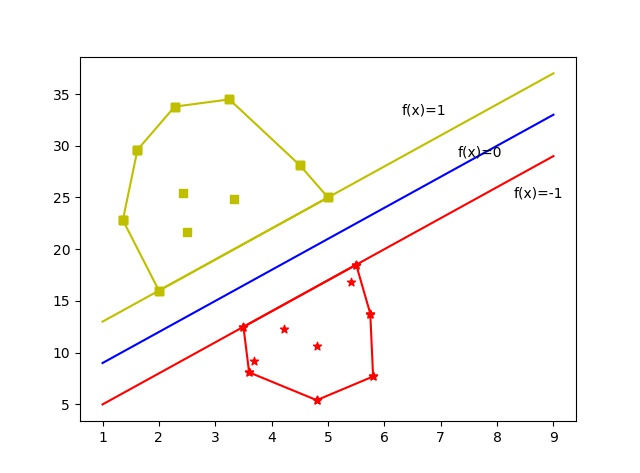
\includegraphics[width=9cm,height=6cm]{HullVector_SupportVector}
  \caption{Relationship between hull vectors and support vectors}
\end{figure}





% 方法
\subsection{Methods}
% 样品制备
\subsubsection{Sample Preparation}
% 谱图采集
\subsubsection{Spectrum acquisition}

% 数据处理
\subsection{Data processing}


%=============第三部分 数据分析===================
\section{III. Data Analysis}
% 拉曼数据分析
\subsection{Raman spectrum Data analysis}
Raman spectroscopy can quickly obtain sample information about the functional groups in aromatic compounds,and has significant advantages: sample preparation is simple, measurement usually does not destroy sample, and moisture does not affect test.

Raman spectrum of Apple essence samples is normally very complex and rich of information of functional group of organic compounds.The Raman spectra mainly reflected the solvent information of the essence, and the Raman spectra of the essence with the same solvent are extremely similar and difficult to be identified manually,as shown in Figure 1.The spectra of essences e, Q, and s are similar,and i,a,c,d,f is similar.The spectra B has more peaks,and contains the peaks of the previous two types of spectra.According to the literature[23] and comparison of standards,the spectra of essences e, Q, and s are the peak of

%=============第四部分 结果与分析===================
\section{IV. Result and Discussion}
The  model  takes  the  whole  Raman  spectrum  and  selects  discernable  features  from the  spectrum.  Later  on  the  model  uses  those  features  for  predicting  unknown  samples.  The developed model has been evaluated by using 10-fold cross validation approach. It basically divided  the  whole  data  set  into10-subsets.  Each  time  the  model  is  trained  on  9  subsets  and tested  on  the  remaining  one.  The  overall  process  is  repeated  10-times,  to  predict  all  the samples stepwise. The beauty of this method is that it does not care about how the data set are divided, because each data must come k-1 times in the training set and once in test set.
\begin{figure}[h]
  \centering
  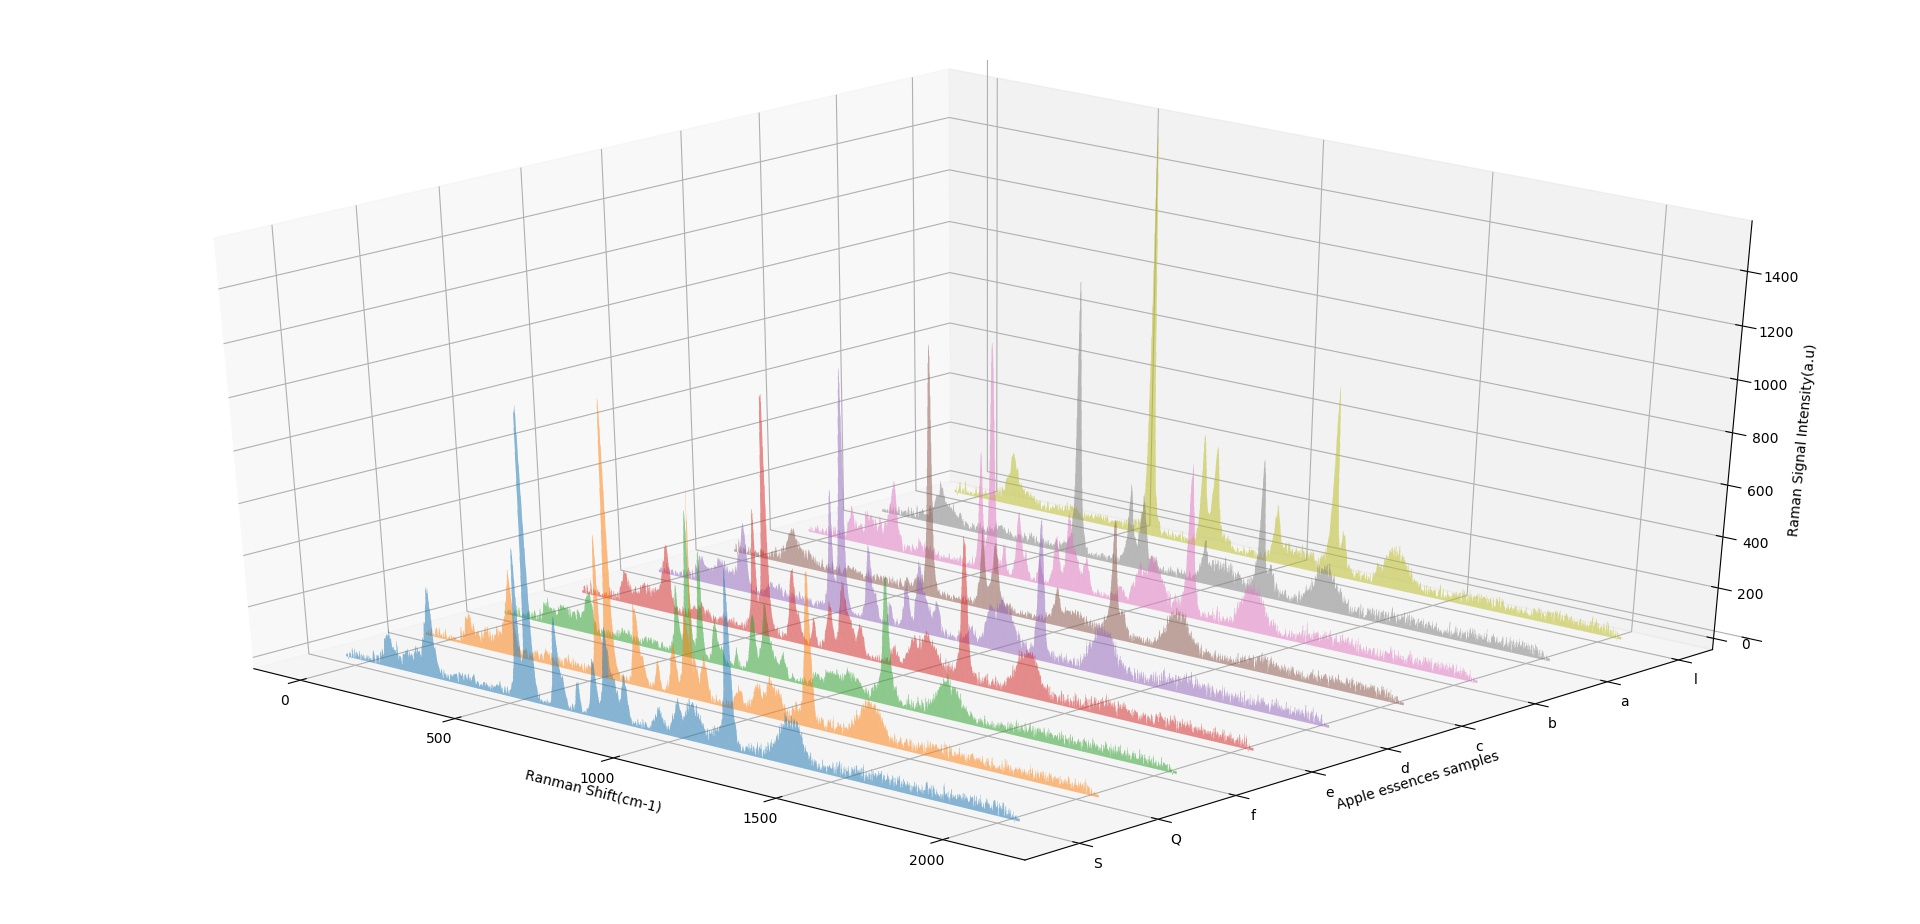
\includegraphics[width=9cm,height=6cm]{Typical_Raman_spectra}
  \caption{Typical Raman spectra of nine kinds of apple essences}
\end{figure}
The overall results for the model with different kernel functions are given in Table 1. The best  performance  has  been  obtained  with  the  polynomial  kernel  function  of  order  1.  The performance  of  a  model  is  usually  evaluated  in  terms  of  accuracy,  precision,  sensitivity  and specificity.  Sensitivity  correctly  sorts  out  all  patients  with  the  disease,  whereas  specificity correctly identifies all patients who do not have that disease [29]. A laboratory test with high specificity and sensitivity is usually desired, but rarely both of these conditions are met at the same time. The aforementioned four parameters for the current SVM model with polynomial kernel function of order 1 have been found 85%, 90%, 73% and 93%, respectively.

%不同香精中化学成分及相对含量不尽相同,组分化合物间也会发生不同的缔合作用,
The chemical components and relative contents of different flavors are different,these will produce different associations,so it  determine the spectral curves of different flavors are somewhat different,and has different  characteristics and fingerprints.The difference between the spectra is the variation of relative intensities of the absorption peaks in the fingerprint region,and the Minute difference in the small peaks in the fingerprint region.Pattern recognition algorithm can maximize the information extracted from the data,and can classify the sample set.

为了进行比较,对3种不同算法进行了仿真.算法1采用标准SVM算法,即在每次增量学习时都使用所有样本求解支持向量进行分类;算法2利用支持向量集代替原样本集进行增量学习,即利用原分类器的支持向量集代替原样本集,再结合新增样本一起进行计算;算法3为本文提出的壳向量增量学习算法.初始样本集为从全部样本中随机选取的135个样本,然后每次加入70个样本,先后共进行3次增量学习,每次增量学习完成后,用全部的345个样本来检验分类效果.计算结果如表1所示.在第1~ 3次增量学习过程后,原有壳向量集与新的壳向量集相比,壳向量转化为非壳向量的个数分别为14、17、18.

For comparison, three different algorithms were simulated.Algorithm A uses the standard SVM algorithm, which uses all the samples to solve the support vector for each incremental learning.Algorithm B uses the support vector set instead of the original sample set for incremental learning,Algorithm 2 uses the support vector set instead of the original sample set for incremental learning, that is,using the original classifier support vector set instead of the original sample set, combined with the new sample to be calculated together.Algorithm 3 is a shell vector incremental learning algorithm.The initial sample set is 135 samples randomly selected from all samples, and 70 samples are added for each incremental learning. After each learning, using all 345 samples to check the classification effect.The results are shown in Table 2,after the first to third incremental learning process,Compared with the new shell vector set, the number of shell vectors transformed into non-shell vectors is 14,17,18.

从仿真结果可以看出,随着增量学习的不断进行,基于壳向量的SVM增量学习算法与标准SVM方法相比,大大地节约了计算时间,加快了仿真速度,而分类正确率基本一致;与利用原分类器的支持向量集代替原样本集,再结合新增样本一起进行计算的方法相比,在计算时间上相差不大,但是提高了分类正确率.因此,本文算法是非常有效的.同时,随着增量学习的不断进行,该算法可以很自然地使部分壳向量转化为非壳向量,从而实现对训练历史数据进行有选择的遗忘.另外还可以看出,当处理样本数目较多的训练集时,增量式壳向量SVM方法的速度优势表现得更为明显。

It can be seen from the simulation results that the SVM incremental learning algorithm based on shell vector is compared with the standard SVM method, which greatly saves the computation time and accelerates the simulation speed, and the classification accuracy is basically the same,the algorithm, that combined the original support vector set with the new sample set rather than an initial sample set,greatly saves the computation time and accelerates the simulation speed, and the classification accuracy is basically the same.Meanwhile, with the continuous learning of incremental learning, the algorithm can naturally make part of the Hull vector into non-Hull vector, to achieve the selective forgetting of the historical data of the training.Therefore, when dealing with a large number of online data set ,the speed advantage of the incremental hull SVM method is more obvious.

\begin{table}[h] %开始一个表格environment,表格的位置是h,here
  \centering
  \caption{Simulation results after adding group samples}\label{a}
  \begin{tabular}{|p{3.5cm}|c|p{1.5cm}|c|c|c|c|}

     \hline
     % after \\: \hline or \cline{col1-col2} \cline{col3-col4} ...
     learning process       & algorithm       & Simulation sample   & Hv    & Sv & t/s    & $\eta$  \\
     \hline
     \multirow{3}{3cm} {Initialization(randomly selected 135 sample data)}&1    &135 & - &34 & 37.5 & 85.80         \\
                                                                       &2    &135 & - &34 & 37.5 & 85.80         \\
                                                                       &3    &135 & - &34 & 37.5 & 85.80         \\

    \hline
     \multirow{3}{3.5cm}{After the first incremental study(add 70 sample data)} &1    &135 & - &34 & 37.5 & 85.80         \\
                                                                       &2    &135 & - &34 & 37.5 & 85.80         \\
                                                                       &3    &135 & - &34 & 37.5 & 85.80         \\
    \hline
    \multirow{3}{3.5cm} {After the second incremental study(add 70 sample data)} &1    &135 & - &34 & 37.5 & 85.80         \\
                                                                       &2    &135 & - &34 & 37.5 & 85.80         \\
                                                                       &3    &135 & - &34 & 37.5 & 85.80         \\
    \hline
    \multirow{3}{3.5cm} {After the third incremental study(add 70 sample data)} &1    &135 & - &34 & 37.5 & 85.80         \\
                                                                       &2    &135 & - &34 & 37.5 & 85.80         \\
                                                                       &3    &135 & - &34 & 37.5 & 85.80         \\
    \hline
  \end{tabular}

\end{table}

%=============第五部分 结论===================
\section{V.	Conclusion}
This  study  demonstrates  the  use  of  Raman  spectroscopy  combined  with Convex-Hull SVM  technique  for the  classification  of  the  spectral  data  acquired  from  Apple essense. Raman  spectroscopy  coupled  with  statistical  tools  has  great  potential  to  contribute significantly in the On-line inspection and research of product quality in an effective way.There is also a great  likelihood  to  use  Raman  spectroscopy  combined  with  one  of  the  existing  methods  for initial screening in order to increase the inspection efficiency. The results obtained are quite promising and interesting. The research work in our laboratory is still in progress striving for increasing sensitivity as well as specificity.

\renewcommand\refname{References}
\begin{thebibliography}{99}
    \bibitem{Vapnik}V.N. Vapnik, The Nature of Statistical Learning Theory, Springer, New York,1995, 8 (6) :988 - 999
    \bibitem{Stefan}Stefan Ruping,Incremental Learning with Support Vector Machines,Technical Reports,2001,228(4):641-642
    \bibitem{XIAORong}XIAO Rong, WANG Ji-cheng, SUN Zheng-xing. Anapproach to incremental SVM learning algorithm.Journal of Nanjing University, 2002, 38(2): 152 157.
    \bibitem{Zhu X}Zhu X, Lafferty J, Ghahramani Z. Combining active learning and semi-supervised learning using Gaussian fields  and  harmonic  functions[C].  In:  Proc  of  ICML  2003  Workshop  on  the  Continuum  from  Labeled  to Unlabeled Data. Menlo Park, CA:AAAI Press,2003:58-65.
    \bibitem{yunjungShin}Hyunjung Shin, Sungzoon Cho, Invariance of neighborhood relation underinput space to feature space mapping, Pattern Recognition Letters, 26 (2005)707–718.
    \bibitem{YJLee}Y.J. Lee, S.Y. Huang, Reduced support vector machines: a statistical theory,IEEE Transactions on Neural Networks 18 (No.1) (2007) 1–13.
\end{thebibliography}


\end{document}

